\documentclass[11pt]{amsart}
\usepackage[margin=1.15in]{geometry}
\usepackage{amsmath,amssymb,amsthm,mathtools}
\usepackage{graphicx}
\usepackage[T1]{fontenc}
\usepackage{lmodern}
\usepackage{microtype}
\usepackage{enumitem}
\usepackage[hidelinks,pdfusetitle]{hyperref}

\newtheorem{theorem}{Theorem}[section]
\newtheorem{lemma}[theorem]{Lemma}
\newtheorem{proposition}[theorem]{Proposition}
\newtheorem{corollary}[theorem]{Corollary}
\newtheorem*{theoremA}{Theorem A}
\newtheorem*{theoremB}{Theorem B}
\newtheorem*{theoremC}{Theorem C}
\newtheorem*{theoremD}{Theorem D}
\newtheorem*{theoremE}{Theorem E}
\theoremstyle{definition}
\newtheorem{definition}[theorem]{Definition}
\newtheorem{problem}[theorem]{Problem}
\newtheorem{example}[theorem]{Example}
\theoremstyle{remark}
\newtheorem{remark}[theorem]{Remark}

\newcommand{\R}{\mathbb{R}}
\newcommand{\Z}{\mathbb{Z}}
\newcommand{\C}{\mathbb{C}}
\newcommand{\SU}{\mathrm{SU}}
\newcommand{\SO}{\mathrm{SO}}
\newcommand{\U}{\mathrm{U}}
\newcommand{\g}{\mathfrak{g}}
\newcommand{\Tr}{\operatorname{Tr}}
\newcommand{\ReTr}{\operatorname{Re}\operatorname{Tr}}
\newcommand{\Hess}{\operatorname{Hess}}
\newcommand{\Ric}{\operatorname{Ric}}
\newcommand{\Cov}{\operatorname{Cov}}
\newcommand{\Var}{\operatorname{Var}}
\newcommand{\dist}{\operatorname{dist}}
\newcommand{\diam}{\operatorname{diam}}
\newcommand{\supp}{\operatorname{supp}}
\newcommand{\ip}[2]{\langle #1,#2\rangle}

\begin{document}

\title{Sharp Curvature and Finite-Box Criteria for Lattice Yang--Mills Theory}

\author{Deep Bhattacharjee}
\address{Formerly, Electro-Gravitational Space Propulsion Laboratory (EGSPL),
Bhubaneswar, Odisha 751030, India}
\address{Formerly, University of Calcutta, Senate House, 87/1 College Street,
Kolkata 700073, West Bengal, India}
\email{d.bhattacharjee@erl-forschung.de}
\email{itsdeep@live.com}
\urladdr{https://orcid.org/0000-0003-0466-750X}
\thanks{Corresponding author: Deep Bhattacharjee.}

\author{Ushashi Bhattacharya}
\address{Formerly, National Taiwan University, Taipei 106319, Taiwan}
\email{rai.bhattacharya.in@gmail.com}

\subjclass[2020]{Primary 81T25 (Quantum field theory on lattices); Secondary
82B20 (Lattice systems and systems on graphs in equilibrium statistical
mechanics), 60K35 (Interacting random processes; statistical mechanics type
models), 58J65 (Diffusion processes and stochastic analysis on manifolds)}
\keywords{lattice gauge theory, Bakry--\'Emery criterion, Dobrushin uniqueness,
mass gap}
\date{18 October 2026}

\begin{abstract}
The Riemannian Hessian of the Wilson action on $d$-dimensional lattice gauge
fields with values in $\SU(N)$, $\SO(N)$ or $\U(N)$ is bounded by $4d$, and the
bound is attained. Consequently the lattice Yang--Mills measure satisfies a
log-Sobolev inequality uniform in the volume for $|\beta|<1/(8d)$, no uniform
curvature argument reaches further, and the $\SU(2)$ Gibbs state is unique for
$|\beta|<1/(8(d-1))$. We also prove a gauge-invariant finite-box criterion for
decay of correlations, and we isolate what is still missing for a mass gap at
intermediate coupling.
\end{abstract}

\maketitle

\section{Introduction}

Wilson's lattice gauge theory~\cite{Wil74} with compact structure group $G$ is
the standard starting point for a construction of four-dimensional Yang--Mills
theory. At strong coupling, that is for small inverse coupling $\beta$, the
theory is under control: the Osterwalder--Seiler cluster
expansion~\cite{OSei78,Sei82} gives a transfer-matrix gap and exponential
clustering, and Shen, Zhu and Zhu~\cite{SZZ23} obtained a log-Sobolev
inequality, uniform in the volume, by verifying the Bakry--\'Emery
criterion~\cite{BE85,BGL14} on the product of copies of $G$. Their argument
rests on a bound
\begin{equation}\label{eq:szzbound}
|\Hess S_0(v,v)|\le 8(d-1)\,|v|^2
\end{equation}
for the Hessian of the Wilson action $S_0=\sum_p\ReTr Q_p$, and gives the
regime $|\beta|<1/(16(d-1))$ in their normalisation. The same constant
$8(d-1)$ is used in later work on the Langevin dynamics, the Yang--Mills--Higgs
model and the 't~Hooft regime~\cite{CNS25b,Nis25,SSZ26}.

The first purpose of this paper is to determine the best constant
in~\eqref{eq:szzbound}. The cross terms between the four links of one
plaquette, which are bounded plaquette by plaquette in~\eqref{eq:szzbound},
reassemble over the whole lattice into the square of a covariant divergence.
This yields the following.

\begin{theoremA}[Sharp Hessian bound]
Let $G\in\{\SU(N),\SO(N),\U(N)\}$ and $d\ge2$. For every gauge field $Q$ on
$\Z^d$ or on a torus and every finitely supported tangent vector
$v=(X_eQ_e)_e$,
\[
\pm\Hess S_0(v,v)+\sum_x|D_xX|^2\le 4d\,|v|^2,
\qquad\text{in particular}\qquad |\Hess S_0(v,v)|\le 4d\,|v|^2,
\]
where $D_xX$ is the covariant divergence~\eqref{eq:divergence}. For every
$N\ge2$ and $d\ge2$ the constant $4d$ is attained with both signs.
\end{theoremA}

For $d=2$ the constants $4d$ and $8(d-1)$ coincide; for $d=3$ and $d=4$ they
are $12$ against $16$ and $16$ against $24$. Within the literature we searched
(arXiv and journals to October 2026) no source states the bound $4d$.

\begin{theoremB}[Strong-coupling regime]
Let $G=\SU(N)$ and $|\beta|<1/(8d)$, or $G=\SO(N)$ with $N\ge3$ and
$|\beta|<(N-2)/(16dN)$. Then the finite-volume Wilson measures satisfy the
Bakry--\'Emery condition with a constant $K>0$ independent of the volume, the
boundary condition and the configuration, and therefore a log-Sobolev and a
Poincar\'e inequality with constants independent of the volume and the
boundary condition. Every infinite-volume limit has exponentially decaying
correlations of local functions.
\end{theoremB}

At $d=4$ the regime is $\beta_W<1/8$ for $\SU(2)$ and $\beta_W<9/32$ for
$\SU(3)$ in the usual Wilson normalisation $\beta_W=N^2\beta$, against
$\beta_W<1/12$ and $\beta_W<3/16$ from~\eqref{eq:szzbound}.

\begin{theoremC}[Limit of the curvature method]
For $G=\SU(N)$ on any even torus,
\[
\inf_Q\lambda_{\min}\bigl(\Ric-N\beta\Hess S_0(Q)\bigr)=\tfrac N2-4dN|\beta| .
\]
No Bakry--\'Emery argument with a lower bound uniform over configurations, in
the bi-invariant metric, reaches beyond $|\beta|=1/(8d)$.
\end{theoremC}

For $\SU(2)$ a different route goes further. The conditional law of a single
link is a von Mises--Fisher law on the three-sphere, and its spectral gap can
be bounded below uniformly in the concentration.

\begin{theoremD}[Uniqueness for $\SU(2)$]
For $G=\SU(2)$ and $|\beta|<1/(8(d-1))$ the Wilson theory on $\Z^d$ has
exactly one infinite-volume Gibbs measure. At $d=4$ this is $\beta_W<1/6$.
Single-link Wasserstein--Dobrushin arguments, in the chordal or the geodesic
metric, cannot go beyond $|\beta|=1/(6(d-1))$, that is $\beta_W=2/9$ at $d=4$.
\end{theoremD}

The second purpose is structural. A finite computation at one coupling
implies decay at all scales for spin systems by the Dobrushin--Shlosman
theorem~\cite{DS85}. For gauge fields the natural boundary data are holonomies,
gauge-equivalent boundary conditions must be identified, and the relevant
disagreement is the one that remains after an interior gauge transformation.
Section~\ref{sec:box} sets this up and proves:

\begin{theoremE}[Gauge-invariant finite-box criterion]
For every compact group $G$ and every finite-range gauge-invariant interaction,
the single finite-box inequality of Definition~\ref{def:gds} implies
uniqueness of the infinite-volume Gibbs measure, exponential decay of all
truncated correlations, and the same decay on every sufficiently large torus,
uniformly in its size and in every 't~Hooft twist sector. The box-hereditary
form implies Wilson's area law.
\end{theoremE}

Two-dimensional $\SU(2)$ theory satisfies this criterion at every coupling
(Proposition~\ref{prop:2d}). For four-dimensional $\U(1)$ theory at weak
coupling the criterion must fail, because the theory is massless there by the
theorems of Guth~\cite{Gut80} and Fr\"ohlich--Spencer~\cite{FS82}; this is a
consistency requirement that the criterion meets by construction.

Section~\ref{sec:transfer} records the reduction of a gap at fixed coupling to
a bound on finite tori that is uniform in their size, together with two
structural differences between $\SU(2)$ and $\U(1)$, and Section~\ref{sec:open}
states the one problem that separates all of this from a mass gap at
intermediate coupling. Nothing in this paper proves a mass gap for
four-dimensional Yang--Mills theory, on the lattice at intermediate coupling
or in the continuum. The authors' earlier paper~\cite{BB26} shows that no
inequality uniform in the lattice spacing, stated in lattice units, can produce
the continuum gap; the results here concern fixed spacing.

Figure~\ref{fig:thresholds} places the thresholds on one axis.

\begin{figure}[t]
\centering
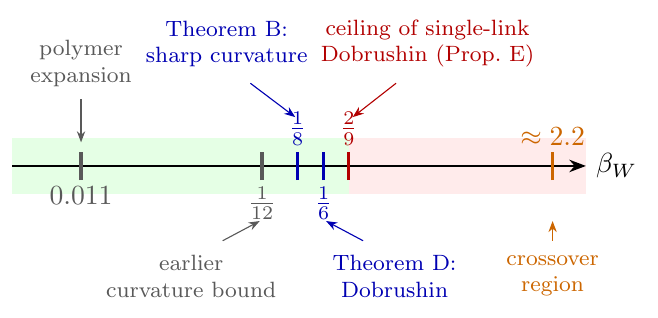
\includegraphics[width=0.92\textwidth]{figures/fig_thresholds.png}
\caption{Strong-coupling thresholds for four-dimensional $\SU(2)$ in the
Wilson normalisation $\beta_W$ (logarithmic scale). Grey: the polymer
expansion and the bound~\eqref{eq:szzbound}. Blue: Theorems~B and~D. Red: the
ceiling of single-link Wasserstein--Dobrushin arguments. Orange: the region
where lattice simulations place the crossover to weak
coupling.\protect\footnotemark}
\label{fig:thresholds}
\end{figure}
\footnotetext{The value $\beta_W\approx2.2$ comes from Monte Carlo
simulations of the string tension and glueball masses; it plays no role in any
proof.}

\section{Setting}\label{sec:setting}

Let $G\in\{\SU(N),\SO(N),\U(N)\}$ with Lie algebra $\g$. We use the inner
product $\ip XY=-\Tr(XY)=\ReTr(X^*Y)$ on $\g$ and the bi-invariant metric it
induces on $G$. In this metric
\begin{equation}\label{eq:ricci}
\Ric_{\SU(N)}=\tfrac N2,\qquad \Ric_{\SO(N)}=\tfrac{N-2}4,
\end{equation}
since $\Ric(X,X)=-\frac14B(X,X)$ for the Killing form $B$, and $B(X,X)=2N\Tr
X^2$ on $\mathfrak{su}(N)$, $B(X,X)=(N-2)\Tr X^2$ on $\mathfrak{so}(N)$. The
group $\SU(2)$ with this metric is the round three-sphere of radius $\sqrt2$.

Let $\Lambda\subset\Z^d$ be a finite box or a torus, $E$ its set of
positively oriented links and $P$ its set of plaquettes. A plaquette $p$ with
base point $x$ in the plane of the directions $\mu<\nu$ has the links
\[
e_1=(x,\mu),\quad e_2=(x+\hat\mu,\nu),\quad e_3=(x+\hat\nu,\mu),\quad
e_4=(x,\nu),
\]
and for $Q\in G^E$ we write $Q_p=Q_{e_1}Q_{e_2}Q_{e_3}^*Q_{e_4}^*$. The Wilson
measure is
\begin{equation}\label{eq:wilson}
d\mu_{\Lambda,\beta}(Q)=Z^{-1}\exp\bigl(S(Q)\bigr)\prod_e dQ_e,\qquad
S=N\beta\,S_0,\qquad S_0(Q)=\sum_{p\in P}\ReTr Q_p,
\end{equation}
with normalised Haar measure $dQ_e$; on a box the links outside $\Lambda$ are
frozen to a boundary condition. This is the normalisation of~\cite{SZZ23}.
The Wilson coupling of the physics literature is $\beta_W=N^2\beta$.

A tangent vector at $Q$ is $v=(X_eQ_e)_e$ with $X_e\in\g$, and
$|v|^2=\sum_e|X_e|^2$. Since $t\mapsto e^{tX}Q$ is a geodesic,
$\Hess S_0(v,v)=\frac{d^2}{dt^2}S_0\bigl((e^{tX_e}Q_e)_e\bigr)|_{t=0}$.

\section{The sharp Hessian bound}\label{sec:hessian}

\subsection{The Hessian of one plaquette}

Fix a plaquette $p$ and a tangent vector $v=(X_eQ_e)$. Transport the four
link vectors to the base point of $p$:
\begin{equation}\label{eq:transport}
Y_1=X_{e_1},\quad Y_2=Q_{e_1}X_{e_2}Q_{e_1}^*,\quad
Y_3=Q_{e_4}X_{e_3}Q_{e_4}^*,\quad Y_4=X_{e_4},\qquad W=Q_p.
\end{equation}
Then $e^{tX_1}Q_1e^{tX_2}Q_2=e^{tY_1}e^{tY_2}Q_1Q_2$ and
$Q_3^*e^{-tX_3}Q_4^*e^{-tX_4}=Q_3^*Q_4^*e^{-tY_3}e^{-tY_4}$, so the perturbed
plaquette variable is $Q_p(t)=e^{tY_1}e^{tY_2}We^{-tY_3}e^{-tY_4}$. Expanding to
second order in $t$ and using the cyclicity of the trace,
\begin{equation}\label{eq:fp}
\begin{split}
f_p:={}&\frac{d^2}{dt^2}\ReTr Q_p(t)\Big|_{t=0}\\
={}&\sum_{i=1}^4\ReTr(Y_i^2W)+2\ReTr(Y_1Y_2W)+2\ReTr(Y_3Y_4W)\\
&-2\!\!\sum_{\substack{i\in\{1,2\}\\ j\in\{3,4\}}}\!\!\ReTr(Y_iWY_j),
\end{split}
\end{equation}
and $\Hess S_0(v,v)=\sum_pf_p$.

\subsection{The covariant divergence}

The covariant divergence of $X$ at a vertex $x$ is
\begin{equation}\label{eq:divergence}
D_xX=\sum_{\mu=1}^d\Bigl[X_{x,\mu}-Q_{x-\hat\mu,\mu}^*X_{x-\hat\mu,\mu}
Q_{x-\hat\mu,\mu}\Bigr]\in\g .
\end{equation}
Each summand is the vector of a link with an end at $x$, transported to $x$,
with sign $+$ for an outgoing and $-$ for an incoming link. The corner form of
the plaquette $p$ is
\begin{equation}\label{eq:corner}
c_p=2\ip{Y_1}{Y_4}-2\ip{Y_1}{Y_2}+2\ip{Y_2}{WY_3W^*}-2\ip{Y_3}{Y_4}.
\end{equation}

\begin{figure}[t]
\centering
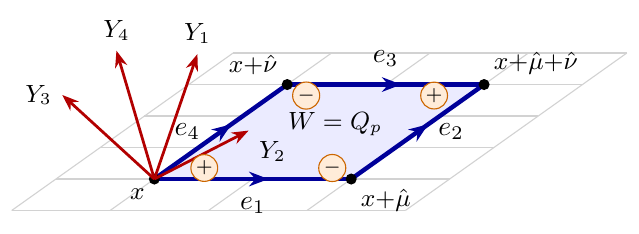
\includegraphics[width=0.7\textwidth]{figures/fig_plaquette.png}
\caption{A plaquette with its links $e_1,\dots,e_4$, the link vectors
$Y_1,\dots,Y_4$ transported to the base point $x$, and the four corners. The
sign at a corner is the sign with which the product of the two link vectors
meeting there enters $|D_yX|^2$ at that vertex $y$, and hence the sign of the
corresponding term of the corner form~\eqref{eq:corner}.}
\label{fig:plaquette}
\end{figure}

\begin{lemma}\label{lem:divergence}
For every configuration $Q$ and every finitely supported $X$,
\[
\sum_x|D_xX|^2=2|X|^2+\sum_pc_p+\sum_{x,\mu}\kappa_{x,\mu},\qquad
\kappa_{x,\mu}=-2\ip{X_{x,\mu}}{Q^*_{x-\hat\mu,\mu}X_{x-\hat\mu,\mu}
Q_{x-\hat\mu,\mu}},
\]
and $\sum_{x,\mu}|\kappa_{x,\mu}|\le 2|X|^2$.
\end{lemma}

\begin{proof}
The vector $D_xX$ is a signed sum of $2d$ vectors, one for each end of a link
at $x$. Expanding $|D_xX|^2$ and summing over $x$ gives three kinds of term.
The squares contribute $2|X|^2$, because every link has two ends. The cross
term of the outgoing and the incoming end in the same direction $\mu$ is
$\kappa_{x,\mu}$. The cross terms of two ends in perpendicular directions
$\mu\ne\nu$ are in bijection with the pairs consisting of a plaquette in the
plane $\mu\nu$ and a corner of it at $x$, since through $x$ pass four
plaquettes of that plane, one for each choice of the two signs.

It remains to identify the four corner terms of a plaquette $p$ with base
point $x$ (Figure~\ref{fig:plaquette}). At $x$ both links are outgoing, which
gives $2\ip{X_{e_1}}{X_{e_4}}=2\ip{Y_1}{Y_4}$. At $x+\hat\mu$ the end of $e_1$
is incoming and $e_2$ is outgoing, which gives $-2\ip{Q_{e_1}^*X_{e_1}Q_{e_1}}
{X_{e_2}}=-2\ip{Y_1}{Y_2}$ after conjugation by $Q_{e_1}$. In the same way the
corner $x+\hat\nu$ gives $-2\ip{Y_4}{Y_3}$. At $x+\hat\mu+\hat\nu$ both links
are incoming, which gives $2\ip{Q_{e_2}^*X_{e_2}Q_{e_2}}{Q_{e_3}^*X_{e_3}
Q_{e_3}}$; conjugating by $Q_{e_1}Q_{e_2}$ and using $Q_{e_1}Q_{e_2}Q_{e_3}^*
=WQ_{e_4}$ turns it into $2\ip{Y_2}{WY_3W^*}$. The four terms add up to $c_p$.
Finally, $|\kappa_{x,\mu}|\le|X_{x,\mu}|^2+|X_{x-\hat\mu,\mu}|^2$ by the
Cauchy--Schwarz inequality, and summing over $(x,\mu)$ counts every link
twice.
\end{proof}

\subsection{A local inequality}

\begin{lemma}\label{lem:local}
For every $N$, every $W\in\U(N)$ and all $Y_1,\dots,Y_4\in\mathfrak u(N)$,
\[
f_p+c_p\le 2\sum_{i=1}^4|Y_i|^2\qquad\text{and}\qquad
-f_p+c_p\le 2\sum_{i=1}^4|Y_i|^2 .
\]
\end{lemma}

\begin{proof}
Replacing $W$ by $-W$ changes the sign of $f_p$ and leaves $c_p$ unchanged, so
the second inequality follows from the first. Write $W=VDV^*$ with $V$ unitary
and $D=\operatorname{diag}(w_1,\dots,w_N)$, $|w_a|=1$. Replacing every $Y_i$ by
$V^*Y_iV$ leaves both sides unchanged, so we may assume $W=D$. Every term of
$f_p$ and $c_p$ then has one of the forms
\[
\operatorname{Re}\sum_{a,b}(Y_i)_{ab}(Y_j)_{ba}w_a,\quad
\operatorname{Re}\sum_{a,b}(Y_i)_{ab}w_b(Y_j)_{ba},\quad
\operatorname{Re}\sum_{a,b}\overline{(Y_i)_{ab}}(Y_j)_{ab},\quad
\operatorname{Re}\sum_{a,b}\overline{(Y_i)_{ab}}(Y_j)_{ab}w_a\bar w_b .
\]
Since $(Y_i)_{ba}=-\overline{(Y_i)_{ab}}$, each of them couples only the entries
in the positions $(a,b)$ and $(b,a)$. Hence the quadratic form
$F=2\sum|Y_i|^2-f_p-c_p$ is an orthogonal sum of blocks of two kinds: one for
each diagonal position $a$, in the variables $(Y_i)_{aa}=\mathrm iy_i$ with
$y\in\R^4$, and one for each unordered pair $a\ne b$, in the variables
$z_i=(Y_i)_{ab}\in\C$. It suffices to show that each block is nonnegative.

\emph{Diagonal blocks.} Put $w_a=e^{\mathrm i\varphi}$. Substituting
$Y_i=\mathrm iy_i$, $W=e^{\mathrm i\varphi}$ in~\eqref{eq:fp}
and~\eqref{eq:corner} and expanding gives
\[
F_{aa}=(y_1+y_3)^2+(y_2+y_4)^2+(1+\cos\varphi)(y_1+y_2-y_3-y_4)^2\ge0 .
\]

\emph{Pair blocks.} Put $w_a=e^{\mathrm i(\chi+\theta)}$,
$w_b=e^{\mathrm i(\chi-\theta)}$ and $m=\cos\chi$. Since $|Y_i|^2$ contains
$2|z_i|^2$ from the two positions $(a,b),(b,a)$, the block is
$F_{ab}=z^*M z$ with $z=(z_1,\dots,z_4)$ and the Hermitian matrix $M$ whose
diagonal entries are $4+2m\cos\theta$ and whose entries above the diagonal are
\[
\begin{gathered}
M_{12}=M_{34}=2+2me^{-\mathrm i\theta},\quad
M_{13}=M_{24}=-2me^{\mathrm i\theta},\\
M_{14}=-2-2me^{\mathrm i\theta},\quad
M_{23}=-2e^{2\mathrm i\theta}-2me^{\mathrm i\theta}.
\end{gathered}
\]
These are obtained by expanding the eight terms of~\eqref{eq:fp}
and~\eqref{eq:corner} on the $2\times2$ minor in the rows and columns $a,b$.
Every entry is affine in $m$, and a direct comparison shows
$M(-1,\theta)=M(1,\theta+\pi)$. Hence
$M(m,\theta)=\tfrac{1+m}2M(1,\theta)+\tfrac{1-m}2M(1,\theta+\pi)$, and it
suffices to show $M(1,\theta)\succeq0$ for all $\theta$. Substitute
$z=\Delta u$ with $\Delta=\operatorname{diag}(1,e^{\mathrm i\theta/2},
e^{-\mathrm i\theta},e^{-\mathrm i\theta/2})$ and put $c=\cos(\theta/2)$. The
matrix $\Delta^*M(1,\theta)\Delta$ is real:
\[
\Delta^*M(1,\theta)\Delta=\begin{pmatrix}
2+4c^2&4c&-2&-4c\\ 4c&2+4c^2&-4c&-2\\ -2&-4c&2+4c^2&4c\\ -4c&-2&4c&2+4c^2
\end{pmatrix},
\]
and comparing coefficients shows that the corresponding form is
\[
2c^2\bigl(|u_1+u_3|^2+|u_2+u_4|^2\bigr)+(1+c)^2|u_1+u_2-u_3-u_4|^2
+(1-c)^2|u_1-u_2-u_3+u_4|^2\ \ge\ 0 .
\]
For instance, the diagonal coefficient is $2c^2+(1+c)^2+(1-c)^2=2+4c^2$ and
the $(1,3)$ coefficient is $2c^2-(1+c)^2-(1-c)^2=-2$.
\end{proof}

\begin{remark}
The blocks of the ordered positions $(a,b)$ and $(b,a)$ taken separately are
not positive semidefinite (take $w_a=-1$, $w_b=1$). The pairing of $(a,b)$ with
$(b,a)$ through $(Y)_{ba}=-\overline{(Y)_{ab}}$ is what makes the inequality
true.
\end{remark}

\subsection{Proof of Theorem A}

\begin{proof}[Proof of the upper bound]
Every link lies in $2(d-1)$ plaquettes and $|Y_i|=|X_{e_i}|$, so summing
Lemma~\ref{lem:local} over $p$ gives $\sum_p(\pm f_p+c_p)\le4(d-1)|X|^2$. By
Lemma~\ref{lem:divergence},
$\sum_pc_p=\sum_x|D_xX|^2-2|X|^2-\sum\kappa\ge\sum_x|D_xX|^2-4|X|^2$. Hence
\[
\pm\Hess S_0(v,v)=\pm\sum_pf_p\le4(d-1)|X|^2+4|X|^2-\sum_x|D_xX|^2. \qedhere
\]
\end{proof}

\begin{proof}[Proof of sharpness]
Let the torus have even side length, and let $X_{x,\mu}=(-1)^{|x|}\varepsilon_\mu
T$ with $|x|=\sum_\nu x_\nu$, a vector $\varepsilon\in\R^d$ with
$\sum_\mu\varepsilon_\mu=0$, and $T\in\g$.

\emph{The sign $-$.} At the identity configuration $W=1$ and $Y_i=X_{e_i}$,
and~\eqref{eq:fp} becomes $f_p=\Tr\bigl((Y_1+Y_2-Y_3-Y_4)^2\bigr)
=-|Y_1+Y_2-Y_3-Y_4|^2$. For the plaquette at $x$ in the plane $\mu\nu$,
$Y_1+Y_2-Y_3-Y_4=2(-1)^{|x|}(\varepsilon_\mu-\varepsilon_\nu)T$. Each vertex
therefore contributes
$-4|T|^2\sum_{\mu<\nu}(\varepsilon_\mu-\varepsilon_\nu)^2
=-4|T|^2\bigl(d|\varepsilon|^2-(\textstyle\sum_\mu\varepsilon_\mu)^2\bigr)
=-4d|\varepsilon|^2|T|^2$, while it carries $|\varepsilon|^2|T|^2$ of $|X|^2$.
So $\Hess S_0(v,v)=-4d|X|^2$. Moreover $D_xX=2(-1)^{|x|}(\sum_\mu
\varepsilon_\mu)T=0$, so the inequality of Theorem~A is an equality.

\emph{The sign $+$.} Let $z=\operatorname{diag}(-1,-1,1,\dots,1)$, which lies in
$\SU(N)$, $\SO(N)$ and $\U(N)$, and let $Q_{x,\mu}=z^{\sum_{\lambda<\mu}x_\lambda}$.
This is well defined on an even torus because $z^2=1$. For the plaquette at
$x$ in the plane $\mu<\nu$ one finds $Q_{e_1}=Q_{e_3}=z^{\sum_{\lambda<\mu}
x_\lambda}$, $Q_{e_4}=z^{\sum_{\lambda<\nu}x_\lambda}$ and $Q_{e_2}=zQ_{e_4}$, so
every plaquette variable equals $z$. Take the same $X$ with $T\ne0$ supported in
the upper left $2\times2$ block, so that $T$ commutes with $z$ and $zT=-T$. All
transports in~\eqref{eq:transport} and~\eqref{eq:divergence} act trivially on
$T$, every term of~\eqref{eq:fp} changes sign relative to the identity
configuration, and therefore $\Hess S_0(v,v)=+4d|X|^2$ and again $D_xX=0$.
\end{proof}

\section{Consequences of the curvature bound}\label{sec:be}

\begin{proof}[Proof of Theorem B]
By Theorem A, $|\Hess S(v,v)|=N|\beta||\Hess S_0(v,v)|\le4dN|\beta||v|^2$. The
Ricci curvature of the product manifold $G^E$, or of $G^{E_{\rm int}}$ with the
boundary links frozen, equals $\Ric_G$ in every direction. By~\eqref{eq:ricci},
\[
\Ric-\Hess S\ \ge\ K:=\tfrac N2-4dN|\beta|\quad(\SU(N)),\qquad
K:=\tfrac{N-2}4-4dN|\beta|\quad(\SO(N)),
\]
uniformly in the volume, the boundary condition and the configuration, and
$K>0$ in the stated ranges. The Bakry--\'Emery criterion on a compact
Riemannian manifold~\cite[Cor.~5.7.2]{BGL14} gives the log-Sobolev inequality
$\operatorname{Ent}_\mu(f^2)\le\frac2K\mu|\nabla f|^2$ and the Poincar\'e
inequality with constant $1/K$.

For the decay of correlations we follow~\cite[\S4]{SZZ23}. The argument there
uses the Langevin dynamics of the Wilson measure and the gradient bound
$|\nabla P_tf|\le e^{-Kt}P_t|\nabla f|$, which is equivalent to the
Bakry--\'Emery condition with constant $K$; the Hessian bound enters only
through the value of that constant. With $K$ in place of the constant
$K_S=\frac N2-8N|\beta|(d-1)$ of~\cite{SZZ23}, the proofs of
\cite[Cor.~4.11 and Rem.~4.12]{SZZ23} apply without change and give exponential
decay of the covariance of local functions, uniformly in the volume, for every
infinite-volume limit.
\end{proof}

\begin{remark}
For $\SU(2)$, uniqueness of the infinite-volume measure in the whole range of
Theorem~B follows from Theorem~D, whose range $1/(8(d-1))$ is larger. For
$\SU(N)$ with $N\ge3$ and for $\SO(N)$ the uniqueness argument of
\cite[\S5]{SZZ23} uses a separate estimate with its own constant, and we do not
claim uniqueness on the whole range $|\beta|<1/(8d)$.
\end{remark}

\begin{proof}[Proof of Theorem C]
By Theorem~A, $(\Ric-N\beta\Hess S_0)(v,v)\ge(\frac N2-4dN|\beta|)|v|^2$ for
every configuration and every $v$, so the infimum is at least
$\frac N2-4dN|\beta|$. For the reverse inequality we may assume $\beta\ne0$ and
take the vector field $v$ of the proof of sharpness. If $\beta>0$ we use the
frustrated configuration, at which $\Hess S_0(v,v)=4d|v|^2$; if $\beta<0$ we use
the identity configuration, at which $\Hess S_0(v,v)=-4d|v|^2$. In both cases
$N\beta\Hess S_0(v,v)=4dN|\beta||v|^2$. The bi-invariant metric on $\SU(N)$ is
Einstein, so $\Ric(v,v)=\frac N2|v|^2$, and therefore
$(\Ric-N\beta\Hess S_0)(v,v)=(\frac N2-4dN|\beta|)|v|^2$.
\end{proof}

A constant rescaling of the metric on all links multiplies $\Ric$ and $\Hess
S$ by the same factor, and a link-dependent constant rescaling does not change
the infimum on a torus, by translation invariance of the extremal
configurations. Theorem~C is a statement about the method; it does not say
that anything changes in the theory at $|\beta|=1/(8d)$.

\section{Uniqueness for SU(2)}\label{sec:su2}

\subsection{The single-link law}

Identify $\SU(2)$ with the unit quaternions, so that $\ReTr U=2x_0(U)$. Fix a
link $e$ and all other links. The action depends on $Q_e$ through
$N\beta\ReTr(Q_eA)$, where $A$ is the sum of the $2(d-1)$ staples of $e$, each
an element of $\SU(2)$, so $A$ corresponds to a vector of $\R^4$ of length at
most $2(d-1)$. The conditional law of $Q_e$ is therefore a von Mises--Fisher law
\[
\nu_\kappa(dx)\propto e^{\kappa x_1}\sigma(dx)\qquad\text{on the unit sphere }
S^3\subset\R^4,
\]
in coordinates in which the staple direction is the $x_1$ axis, with
concentration $\kappa=4|\beta||A|$ (and $x_1$ replaced by $-x_1$ if
$\beta<0$).

\begin{lemma}\label{lem:vmf}
For every $\kappa\ge0$ the spectral gap of $\nu_\kappa$ on the unit sphere $S^3$
is at least $3$, with equality at $\kappa=0$. On the sphere of radius
$\sqrt2$, which is $\SU(2)$ in the metric of Section~\ref{sec:setting}, it is at
least $3/2$.
\end{lemma}

\begin{proof}
Let $\theta\in(0,\pi)$ be the polar angle from the $x_1$ axis. The generator of
the reversible diffusion for $\nu_\kappa$ is
\[
L=\partial_\theta^2+b\,\partial_\theta+\sin^{-2}\theta\,\Delta_{S^2},\qquad
b=2\cot\theta-\kappa\sin\theta=\frac{w'}{w},\quad w=\sin^2\theta\,
e^{\kappa\cos\theta}.
\]
On spherical harmonics of degree $\ell$ on $S^2$ it acts as the
Sturm--Liouville operator $L_\ell=w^{-1}\partial_\theta(w\partial_\theta)-
\ell(\ell+1)\sin^{-2}\theta$ on $L^2((0,\pi),w\,d\theta)$.

We use the ground-state bound of Barta~\cite{Bar37}. Let
$\mathcal L=w^{-1}\partial(w\partial)-q$ with $q$ continuous on $(0,\pi)$, let
$\psi>0$ be smooth on $(0,\pi)$ with $-\mathcal L\psi\ge c\psi$, and let $f$ be
smooth with compact support in $(0,\pi)$. Writing $f=\psi h$ and integrating
by parts,
\[
\int_0^\pi\bigl(f'^2+qf^2\bigr)w\,d\theta=\int_0^\pi\psi^2h'^2w\,d\theta
+\int_0^\pi(-\mathcal L\psi)\psi h^2w\,d\theta\ \ge\ c\int_0^\pi f^2w\,d\theta .
\]
When $q\ge 2\sin^{-2}\theta-C$ near the endpoints, compactly supported functions
form a core for the quadratic form, and the bound holds for the lowest point of
the spectrum of $-\mathcal L$.

\emph{Degrees $\ell\ge1$.} Here $q=\ell(\ell+1)\sin^{-2}\theta$ increases with
$\ell$, so it suffices to take $\ell=1$. With $\psi=\sin\theta\,
e^{a\kappa\cos\theta}$ a direct differentiation gives
\[
-\frac{L_1\psi}{\psi}=3+(5a+1)\kappa\cos\theta-a(a+1)\kappa^2\sin^2\theta,
\]
and for $a=-\frac15$ this equals $3+\frac4{25}\kappa^2\sin^2\theta\ge3$.

\emph{Degree $\ell=0$.} Let $g$ be a nonconstant zonal eigenfunction,
$L_0g=-\lambda g$, and put $h=g'$. Then $h(0)=h(\pi)=0$, and differentiating
the eigenvalue equation gives $h''+bh'+b'h=-\lambda h$, that is
$\mathcal Mh=-\lambda h$ with $\mathcal M=w^{-1}\partial(w\partial)+b'$ and
$-b'=2\sin^{-2}\theta+\kappa\cos\theta$. With the same $\psi$,
\[
-\frac{\mathcal M\psi}{\psi}=3+(5a+2)\kappa\cos\theta-a(a+1)\kappa^2
\sin^2\theta,
\]
and for $a=-\frac25$ this equals $3+\frac6{25}\kappa^2\sin^2\theta\ge3$. Hence
$\lambda\ge3$.

At $\kappa=0$ the gap of $S^3$ is $3$. Rescaling the radius from $1$ to
$\sqrt2$ divides eigenvalues by $2$.
\end{proof}

\subsection{Proof of Theorem D}

Let $\rho$ be the geodesic distance on $\SU(2)$ in the metric of
Section~\ref{sec:setting}. For links $e\ne e'$ the Dobrushin coefficient is
\[
C_{ee'}=\sup\frac{W_1(\mu_e^\omega,\mu_e^{\omega'})}{\rho(\omega_{e'},
\omega'_{e'})},
\]
where $\mu_e^\omega$ is the conditional law of $Q_e$ given the configuration
$\omega$ off $e$, $W_1$ is the Kantorovich distance for $\rho$, and the
supremum runs over pairs $\omega,\omega'$ that differ only at $e'$.

\begin{proof}
If $e$ and $e'$ do not lie in a common plaquette, $\mu_e^\omega$ does not depend
on $\omega_{e'}$ and $C_{ee'}=0$. Otherwise they lie in exactly one common
plaquette. Join $\omega_{e'}$ to $\omega'_{e'}$ by a unit-speed geodesic
$s\mapsto\omega_{e'}(s)$ and let $\mu_s$ be the corresponding conditional law at
$e$. For a $1$-Lipschitz function $g$,
\[
\frac{d}{ds}\mu_s(g)=\Cov_{\mu_s}(g,\partial_sS),\qquad
|\Cov_{\mu_s}(g,\partial_sS)|\le\bigl(\Var g\,\Var\partial_sS\bigr)^{1/2}
\le\tfrac23\,\|\nabla_eg\|_{L^2}\,\|\nabla_e\partial_sS\|_{L^2},
\]
by the Poincar\'e inequality of Lemma~\ref{lem:vmf}. Only the common plaquette
contributes to $\nabla_e\partial_sS$; its mixed second derivative is
$N\beta\ReTr(AWB)$ with unit vectors $A,B\in\mathfrak{su}(2)$ and $W\in\SU(2)$,
so $|\nabla_e\partial_sS|\le N|\beta|=2|\beta|$. Integrating in $s$ and taking
the supremum over $g$ (Kantorovich--Rubinstein duality) gives
$C_{ee'}\le\frac43|\beta|$. A link lies in $2(d-1)$ plaquettes, each with three
other links, so
\[
\alpha:=\sup_e\sum_{e'}C_{ee'}\le6(d-1)\cdot\tfrac43|\beta|=8(d-1)|\beta|.
\]
For $\alpha<1$ Dobrushin's uniqueness theorem for compact metric spin spaces
with the Kantorovich distance~\cite{Dob70,DSa23} gives uniqueness of the
infinite-volume Gibbs measure.
\end{proof}

\begin{remark}
Dobrushin's condition also gives decay of correlations of Lipschitz local
functions at rate $\log(1/\alpha)$ per unit distance~\cite{Fol82}. For $\SU(N)$
with $N\ge3$ the staple sum is not a multiple of a unitary matrix, and the same
argument with the single-link Bakry--\'Emery bound reproduces only
$|\beta|<1/(16(d-1))$.
\end{remark}

\begin{proposition}[The ceiling]\label{prop:ceiling}
Let $\delta$ be the chordal metric of $S^3\subset\R^4$ or the geodesic metric,
used for both the distance at $e'$ and the Kantorovich distance at $e$. For all
links $e,e'$ in a common plaquette, $C_{ee'}\ge|\beta|$. Hence no argument
through single-link Dobrushin coefficients proves uniqueness beyond
$|\beta|=1/(6(d-1))$.
\end{proposition}

\begin{proof}
The $2(d-1)$ staples of $e$ involve pairwise disjoint sets of links other than
$e'$, so they can be chosen with sum zero while the staple through $e'$ is an
arbitrary unit quaternion. Then $\kappa=0$ and $\mu_e^\omega$ is uniform.
Moving $Q_{e'}$ by a small distance $\varepsilon$ moves the staple sum by an
isometric image of the displacement, since left and right multiplications by
unit quaternions are isometries of $\R^4$. For $h\in\R^4$ the derivative of the
law in the direction $h$ at zero staple is the signed measure
$4\beta\ip xh\sigma(dx)$. Testing it against the $1$-Lipschitz function
$x\mapsto\ip x{\hat h}$ gives
$4|\beta||h|\int\ip x{\hat h}^2d\sigma=|\beta||h|$, since
$\int x_1^2\,d\sigma=\frac14$ on $S^3$. Hence $C_{ee'}\ge|\beta|$, and summing
over the $6(d-1)$ neighbours gives $\alpha\ge6(d-1)|\beta|$.
\end{proof}

\begin{remark}
In the chordal metric the reflection coupling
$x\mapsto x-2\ip x{\hat h}\hat h$ shows that $|\beta|$ is the exact value at
zero staple. A 2026 preprint attributed to J.~Lockwood, which we have seen only
as an abstract, announces uniqueness for four-dimensional $\SU(2)$ at
$\beta_W<2/9$ by the Wasserstein--Dobrushin method. By
Proposition~\ref{prop:ceiling} that value is exactly the ceiling of the method,
and it would follow if the Lipschitz constant of the von Mises--Fisher family
on $S^3$ were largest at zero concentration. We have not been able to check that
claim.
\end{remark}

\section{A gauge-invariant finite-box criterion}\label{sec:box}

\subsection{Interactions and boundary data}

Let $G$ be a compact metrisable group with normalised Haar measure $\lambda$,
and let $E$ be the set of positively oriented links of $\Z^d$ or of a torus.
An interaction is a family $\Phi=(\Phi_X)$ indexed by finite sets $X\subset E$
of diameter at most $R$, with $\Phi_X\colon G^X\to\R$ continuous, invariant
under translations, and gauge invariant: $\Phi_X(gU)=\Phi_X(U)$ for every
$g\colon\Z^d\to G$, where $(gU)_{xy}=g_xU_{xy}g_y^{-1}$. The Wilson action is
$\Phi_p=-N\beta\ReTr U_p$; a renormalised effective action adds further terms.

For finite $V\subset E$ let $\partial V=\bigcup\{X\setminus V:X\cap V\ne
\emptyset,\ \Phi_X\not\equiv0\}$. The specification is
\[
\gamma_V(dU_V\mid\omega)=Z_V(\omega)^{-1}\exp\Bigl(-\sum_{X\cap V\ne\emptyset}
\Phi_X(U_V\omega)\Bigr)\lambda^V(dU_V),
\]
and it depends on $\omega$ only through $\omega_{\partial V}$. Let $I(V)$ be the
set of vertices all of whose incident links lie in $V$, and $\mathcal G_V=
G^{I(V)}$. A gauge transformation at $x\in I(V)$ moves only links of $V$, so
\begin{equation}\label{eq:interiorinv}
g_*\gamma_V(\cdot\mid\omega)=\gamma_V(\cdot\mid\omega)\qquad(g\in\mathcal G_V).
\end{equation}

\begin{lemma}\label{lem:quotient}
Let $\Gamma_V$ be the graph with edge set $\partial V$. If
$\omega'_{\partial V}=(h\omega)_{\partial V}$ for a map $h$ from the vertices of
$\Gamma_V$ to $G$, then $\gamma_V(\cdot\mid\omega')=(\tilde h|_V)_*\gamma_V(
\cdot\mid\omega)$ for any extension $\tilde h$ of $h$. Consequently
gauge-invariant expectations $\gamma_V(F\mid\omega)$ depend only on the class of
$\omega_{\partial V}$ in $G^{\partial V}/G^{\mathrm{vert}(\Gamma_V)}$, which for
each connected component of $\Gamma_V$ is the space of holonomy representations
of its fundamental group modulo conjugation. (This is the holonomy of the
gauge field; for the holonomy of a Riemannian metric in a related $\SU(n)$
setting see~\cite{BTBS26}.)
\end{lemma}

\begin{proof}
Change variables $U_V\mapsto\tilde hU_V$: Haar measure and the energy are
invariant. For the second statement, gauge the links of a spanning tree of each
component to the identity; the remaining links are free generators of the
fundamental group, and the residual freedom is one constant per component,
acting by conjugation.
\end{proof}

Plaquette holonomies alone do not determine this class when $G$ is
non-abelian; holonomies of larger loops of the shell
enter.\footnote{Take two plaquettes of the shell sharing a vertex, with based
holonomies $(X,Y)$ and $(X,Y')$, where $X=Y=\mathrm i\sigma_3$ and
$Y'=\mathrm i\sigma_1$ in $\SU(2)$. Each holonomy is conjugate to its partner,
but $\Tr(XY)=-2\ne0=\Tr(XY')$, and $XY$ is the holonomy of the boundary of the
union of the two plaquettes.} The criterion below therefore compares boundary
conditions that differ at one link.

\begin{lemma}[Gauge lift]\label{lem:lift}
Let $\Pi$ be a coupling of $\gamma_V(\cdot\mid\omega)$ and
$\gamma_V(\cdot\mid\omega')$, let $g\colon G^V\times G^V\to\mathcal G_V$ be
measurable, and let $h$ be Haar distributed on $\mathcal G_V$, independent of
$(U,U')\sim\Pi$. Then $(hU,\,hg(U,U')U')$ is again a coupling of the two
measures, and $\mathbb P[(hU)_b\ne(hgU')_b]=\Pi[U_b\ne(g(U,U')U')_b]$ for every
link $b$.
\end{lemma}

\begin{proof}
By~\eqref{eq:interiorinv}, $hU\sim\gamma_V(\cdot\mid\omega)$. Given $(U,U')$,
the element $hg$ is Haar distributed, so $hgU'$ is uniform on the
$\mathcal G_V$-orbit of $U'$, and by~\eqref{eq:interiorinv} again
$hgU'\sim\gamma_V(\cdot\mid\omega')$. Each $h_x$ acts on a link by a bijection
of $G$, which preserves equality of the two link values.
\end{proof}

\subsection{The criterion}

Write $V_\mu$ for the links of $V$ in direction $\mu$, $n_{\min}=\min_\mu
|V_\mu|$, and $\omega\sim_y\omega'$ when $\omega,\omega'$ differ only at the link
$y\in\partial V$.

\begin{definition}\label{def:gds}
The interaction satisfies the gauge Dobrushin--Shlosman condition
$\mathrm{GDS}(V,\varepsilon)$ if there are a Borel family of couplings
$\Pi_{\omega,\omega'}$ of $\gamma_V(\cdot\mid\omega)$ and
$\gamma_V(\cdot\mid\omega')$, for all pairs $\omega\sim_y\omega'$, and numbers
\[
\kappa_V(y,b)\ \ge\ \sup_{\omega\sim_y\omega'}\Pi_{\omega,\omega'}[U_b\ne U'_b]
\qquad(y\in\partial V,\ b\in V)
\]
such that for every direction $\nu$
\begin{equation}\label{eq:gds}
K_V(\nu):=\sum_{y\in\partial V,\ \mathrm{dir}\,y=\nu}\ \sum_{b\in V}
\kappa_V(y,b)\ \le\ (1-\varepsilon)\,n_{\min}.
\end{equation}
\end{definition}

By Lemmas~\ref{lem:quotient} and~\ref{lem:lift} the couplings may be
constructed on the gauge quotient and then aligned by any measurable choice of
interior gauge, and the supremum is a supremum over classes of shell holonomies
(Figure~\ref{fig:box}). For a box symmetric under the hypercubic group,
\eqref{eq:gds} reads $\sum_{y,b}\kappa_V(y,b)\le(1-\varepsilon)|V|$, the form
of Dobrushin and Shlosman~\cite{DS85}, except that the supremum over boundary
conditions is taken for each $b$ separately; this is what makes the proof below
work for an arbitrary compact group.

\begin{figure}[t]
\centering
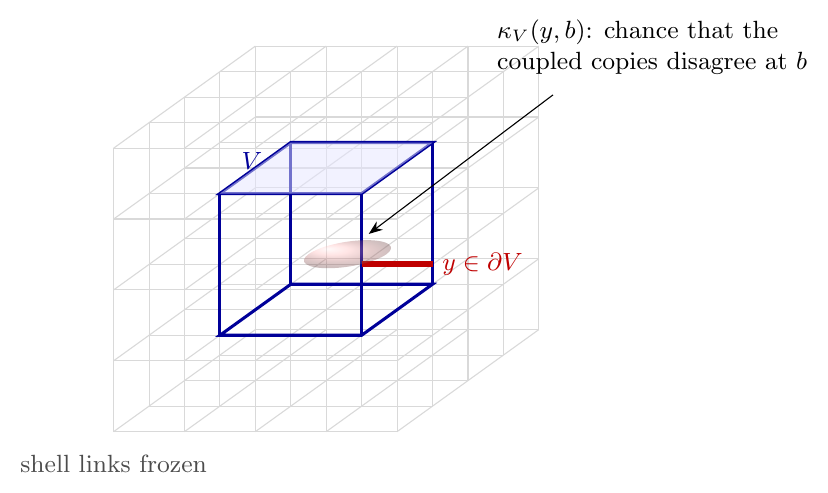
\includegraphics[width=0.62\textwidth]{figures/fig_box.png}
\caption{The box $V$ and a boundary link $y$. Two copies of the box are
coupled, with boundary conditions differing only at $y$; $\kappa_V(y,b)$
bounds the probability that they disagree at $b$ after the best interior gauge
alignment.}
\label{fig:box}
\end{figure}

\begin{theorem}\label{thm:box}
Assume $\mathrm{GDS}(V,\varepsilon)$ for a finite-range gauge-invariant
interaction with compact $G$. Let $D=\max\{|b-y|:b\in V,\ y\in\partial V\}$,
with distances between link midpoints, and $0<\lambda<|\log(1-\varepsilon)|/D$,
so that $\theta:=(1-\varepsilon)e^{\lambda D}<1$. Then:
\begin{enumerate}[label=\textup{(\roman*)}]
\item There is exactly one Gibbs measure $\mu$ on $G^E$; it is invariant under
translations and gauge transformations.
\item Let $S\subset E$ be finite and let $\mu_1,\mu_2$ be probability measures
invariant under $\gamma_{V+a}$ for every translate with $(V+a)\cap S=
\emptyset$. Let $N_S$ be $S$ together with the links of the translates of $V$
that meet $S$; then $|N_S|\le c_V|S|$. There is a coupling of $\mu_1$ and
$\mu_2$ under which, for every link $b$ at distance greater than $\diam V+R$
from $S$,
\[
\mathbb P[\sigma_b\ne\sigma'_b]\le\frac{\theta}{1-\theta}\sum_{z\in N_S}
e^{-\lambda|b-z|}.
\]
\item For bounded $F,H$ with finite supports $S_F,S_H$,
\[
|\Cov_\mu(F,H)|\le2\|F\|_\infty\|H\|_\infty\frac{\theta}{1-\theta}\,c_V
|S_F||S_H|\,e^{-\lambda(\dist(S_F,S_H)-\diam V-R)} .
\]
\item Items \textup{(i)--(iii)} hold on every torus of side greater than
$2(\diam V+R)$ with the same constants, for the untwisted and for every
't~Hooft twisted Wilson action.
\end{enumerate}
\end{theorem}

\begin{proof}
\emph{A minimal coupling.} Let $W$ be $E$ or $E\setminus S$, let $\mathcal A=
\{a:V+a\subseteq W\}$ and $V_a=V+a$. Fix a link $b_0$ and put $w_b=e^{-\lambda
|b-b_0|}$, so that $\sum_bw_b<\infty$. On the set $\mathcal C$ of couplings of
$\mu_1,\mu_2$ define $\Psi(\pi)=\sum_bw_b\,\pi[\sigma_b\ne\sigma'_b]$. The set
$\mathcal C$ is weakly compact because $G^E$ is compact, and each map
$\pi\mapsto\pi[\sigma_b\ne\sigma'_b]$ is lower semicontinuous, being the measure
of an open set. So $\Psi$ attains its minimum at some $\pi^*$. Put
$\rho(b)=\pi^*[\sigma_b\ne\sigma'_b]$.

\emph{Block resampling.} For $a\in\mathcal A$ define a new coupling $T_a\pi^*$:
sample $(\sigma,\sigma')\sim\pi^*$, keep both configurations off $V_a$, and
inside $V_a$ sample from the following path coupling of
$\gamma_{V_a}(\cdot\mid\sigma)$ and $\gamma_{V_a}(\cdot\mid\sigma')$. List
$\partial V_a=\{z_1,\dots,z_k\}$ and let $\omega^j$ agree with $\sigma'$ on
$z_1,\dots,z_j$ and with $\sigma$ elsewhere. Consecutive $\omega^{j-1},\omega^j$
are equal or differ only at $z_j$; couple their block laws by the identity in
the first case and by the translate of $\Pi_{\omega^{j-1},\omega^j}$ in the
second, and chain the couplings through their disintegrations, which depend
measurably on the parameters~\cite[Ch.~3]{Kal21}. This produces
$\tau^0,\dots,\tau^k$ with $\tau^0\sim\gamma_{V_a}(\cdot\mid\sigma)$,
$\tau^k\sim\gamma_{V_a}(\cdot\mid\sigma')$ and $\mathbf 1[\tau^0_b\ne\tau^k_b]
\le\sum_j\mathbf 1[\tau^{j-1}_b\ne\tau^j_b]$. Since each $\mu_i$ is
$\gamma_{V_a}$-invariant, $T_a\pi^*\in\mathcal C$, and for $b\in V_a$
\[
T_a\pi^*[\tau_b\ne\tau'_b]\le\sum_{z\in\partial V_a}\kappa_V(z-a,b-a)\rho(z),
\]
while nothing changes off $V_a$. Minimality, $\Psi(T_a\pi^*)\ge\Psi(\pi^*)$,
gives
\begin{equation}\label{eq:blockineq}
\sum_{b\in V_a}w_b\rho(b)\le\sum_{b\in V_a}w_b\sum_{z\in\partial V_a}
\kappa_V(z-a,b-a)\rho(z).
\end{equation}

\emph{Summation over blocks.} Sum~\eqref{eq:blockineq} over $a\in\mathcal A$;
all series converge, the left side being at most $|V|\sum_bw_b$. Let $W^\circ$
be the set of links $b$ such that every translate of $V$ containing $b$ lies in
$W$; then $E\setminus W^\circ\subseteq N_S$. A link $b$ of direction $\mu$ lies
in exactly $|V_\mu|\ge n_{\min}$ translates. On the right, $|z-b|\le D$ gives
$w_b\le e^{\lambda D}w_z$, and for fixed $z$ of direction $\nu$ the sum over all
$a$ with $z\in\partial V_a$ and all $b\in V_a$ of $\kappa_V(z-a,b-a)$ equals
$K_V(\nu)$. By~\eqref{eq:gds},
\[
n_{\min}\sum_{b\in W^\circ}w_b\rho(b)\le\theta\,n_{\min}\Bigl[\sum_{z\in
W^\circ}w_z\rho(z)+\sum_{z\in N_S}w_z\Bigr],
\]
so $\sum_{W^\circ}w\rho\le\frac{\theta}{1-\theta}\sum_{z\in N_S}w_z$. Taking
$b_0\in W^\circ$ and keeping only the term $b=b_0$ on the left proves (ii).

\emph{Uniqueness.} With $S=\emptyset$, $N_S=\emptyset$ and $\rho\equiv0$, so any
two Gibbs measures coincide. Gibbs measures exist by compactness, and
translates and gauge transforms of a Gibbs measure are Gibbs measures; since
there is only one, it is invariant. This is (i).

\emph{Decay.} Let $\mu^u=\mu(\cdot\mid U_{S_H}=u)$ be a regular conditional
probability; for $\mu$-almost every $u$ it is invariant under every
$\gamma_{V_a}$ with $V_a\cap S_H=\emptyset$. Since $\Cov(F,H)=\int H(u)
[\mu^u(F)-\int\mu^{u'}(F)\mu(du')]\mu(du)$,
$|\Cov(F,H)|\le\|H\|_\infty\operatorname{ess\,sup}_{u,u'}|\mu^u(F)-\mu^{u'}(F)|$,
and $|\mu^u(F)-\mu^{u'}(F)|\le2\|F\|_\infty\sum_{b\in S_F}\rho(b)$. Item (ii)
with $S=S_H$ gives (iii).

\emph{Tori and twists.} On a torus of side greater than $2(\diam V+R)$ every
translate is a genuine block and the argument is unchanged. Let $z_p\in Z(G)$ be
a twist that is closed, so that on every ball of radius at least $\diam V+R$ it
equals $(dn)_p=\prod_{e\in\partial p}n_e^{\pm1}$ for some $n\colon E\to Z(G)$;
every 't~Hooft twist has this property, because a closed $Z(G)$-valued
$2$-cocycle is exact on a contractible ball. Multiplication $M_n$ of each link by
the central element $n_e$ satisfies $\gamma^{\rm tw}_{V_a}(\cdot\mid\omega)=
(M_n)_*\gamma_{V_a}(\cdot\mid M_n\omega)$ on such a ball, since the central
factors commute through, and $M_n$ is a bijection on each link. So the twisted
specification satisfies $\mathrm{GDS}(V,\varepsilon)$ with the same $\kappa_V$,
and the proof applies. This is (iv).
\end{proof}

\subsection{Confinement and stability}

Let $\mathcal V$ be the family of sets $V\cap W'$, where $W'$ runs over the
interior link sets of all cubes in all positions. The box-hereditary condition
$\mathrm{HGDS}(V,\varepsilon)$ is~\eqref{eq:gds} with $\sum_b\kappa_V(y,b)$
replaced by $\sup_{V'\in\mathcal V,\ y\in\partial V'}\sum_{b\in V'}
\kappa_{V'}(y,b)$, the boundary condition of $V'$ including the links of
$V\setminus V'$.

\begin{proposition}\label{prop:hgds}
Assume $\mathrm{HGDS}(V,\varepsilon)$ for the Wilson action of a compact group
$G\subset\U(n)$. Then covariances of local functions under the finite-volume
measure of every cube with every boundary condition decay exponentially with
constants independent of the cube and the boundary condition. By
Chatterjee's theorem~\cite[Thm.~2.4]{Cha21}, the centre symmetry is unbroken
and, if the representation acts non-trivially on the centre, Wilson loops obey
the area law.
\end{proposition}

\begin{proof}
Fix a cube $B$ with boundary condition $\delta$ and interior link set $W_B$,
and local functions $F,H$. Condition $\mu_{B,\delta}$ on $U_{S_H}=u$ and on
$U_{S_H}=u'$, and run the proof of Theorem~\ref{thm:box} in
$W=W_B\setminus S_H$ with all blocks $V_a\cap W_B$ that meet $W$. A link of $W$
of direction $\mu$ now lies in $|V_\mu|\ge n_{\min}$ blocks, so no boundary
layer is lost on the left side of the summed inequality. A link $z\in W$ that
lies in $\partial(V_a\cap W_B)$ lies in $\partial V_a$, and its total weight on
the right is bounded by the hereditary condition. The remaining links of
$\partial(V_a\cap W_B)$ either lie outside $B$, where both copies carry
$\delta$, or lie in $S_H$. So the only sources of disagreement are the links of
$S_H$, each with weight at most $(|V|+|\partial V|)|V|/n_{\min}$ times
$e^{\lambda D}$, and the covariance bound follows as in
Theorem~\ref{thm:box}(iii), uniformly in $B$ and $\delta$. This is the
decay property of~\cite[Def.~2.3]{Cha21}.
\end{proof}

\begin{lemma}\label{lem:stability}
Suppose $\Phi$ satisfies $\mathrm{GDS}(V,\varepsilon)$, and let $\Phi'=\Phi+
\mathcal E$ with $\mathcal E$ gauge invariant of range at most $R$. Put
$t=\tanh\bigl(\frac12\sum_{X\cap V\ne\emptyset}\|\mathcal E_X\|_\infty\bigr)$.
Then $\Phi'$ satisfies $\mathrm{GDS}(V,\varepsilon')$ with $\varepsilon'=
\varepsilon-2t|V|\max_\nu|\partial V|_\nu/n_{\min}$, where $|\partial V|_\nu$
is the number of links of direction $\nu$ in $\partial V$.
\end{lemma}

\begin{proof}
The two energies on $V$ differ by a function of oscillation at most
$s=2\sum_{X\cap V\ne\emptyset}\|\mathcal E_X\|_\infty$. Two probability measures
whose log-densities with respect to a common measure differ by a function of
oscillation $s$ are within total variation $\tanh(s/4)$: if the density ratio
takes values in $[c,ce^s]$, the total variation is at most
$\sup_{0\le x\le1}\bigl(\frac{xe^s}{1+x(e^s-1)}-x\bigr)=\tanh(s/4)$. Glue an
optimal coupling of $\gamma'_V(\cdot\mid\omega)$ with $\gamma_V(\cdot\mid
\omega)$, then $\Pi_{\omega,\omega'}$, then an optimal coupling of
$\gamma_V(\cdot\mid\omega')$ with $\gamma'_V(\cdot\mid\omega')$. Then
$\kappa'(y,b)\le\kappa(y,b)+2t$, and summing over $b\in V$ and $y$ of
direction $\nu$ gives the stated loss.
\end{proof}

The smallness required in Lemma~\ref{lem:stability} shrinks with the box,
since $t$ must be of order $\varepsilon/(|V||\partial V|)$. This matters for
Section~\ref{sec:open}.

\subsection{Two dimensions}

In two dimensions the criterion holds at every coupling. Take $G=\SU(2)$ and
the plaquette weight $w(U)=e^{\frac\beta2\Tr U}$, write $c_0=\int w$, $f=w/c_0$
and $a_j=I_{2j+1}(\beta)/I_1(\beta)$ for $j=\frac12,1,\dots$, where $I_n$ is the
modified Bessel function. The character expansion of $f$ gives
$f^{*m}=\sum_j(2j+1)a_j^m\chi_j$ and
\[
\varepsilon_m:=\sup_U|f^{*m}(U)-1|=\sum_{j\ge1/2}(2j+1)^2a_j^m,
\]
the supremum being attained at the identity because all $a_j$ are positive.
Since $0<a_j<1$ and $\sum_j(2j+1)^2a_j<\infty$, $\varepsilon_m\to0$
exponentially as $m\to\infty$.

\begin{lemma}[Disk integration~\cite{Mig75,Lev03}]\label{lem:disk}
For a simply connected union $D$ of $k$ plaquettes,
$\int\prod_{p\subset D}w(U_p)\,dU_{\mathrm{int}\,D}=c_0^kf^{*k}(\mathrm{hol}_{
\partial D})$.
\end{lemma}

\begin{proof}
Add the plaquettes one at a time in an order in which each new plaquette meets
the region already built in a connected arc $u_1\cdots u_r$. Substituting
$g=u_1\cdots u_r$ and using invariance of Haar measure gives $\int f^{*m}(Ag)
f(g^{-1}B)\,dg=f^{*(m+1)}(AB)$, and the remaining arc variables integrate to
$1$.
\end{proof}

\begin{proposition}\label{prop:2d}
For every $\beta>0$ there is $L$ such that two-dimensional $\SU(2)$ Wilson
theory satisfies $\mathrm{GDS}(V,\varepsilon)$ for the set $V$ of the
$2L(L-1)$ interior links of an $L\times L$ square and some $\varepsilon>0$.
\end{proposition}

\begin{proof}
For $y\in\partial V$ choose an $s\times s$ sub-square $D$ with $y$ on its outer
side; let $L_D$ be its $2s(s-1)$ interior links and $L_R=V\setminus L_D$. By
Lemma~\ref{lem:disk}, under $\gamma_V(\cdot\mid\omega)$ the marginal on $L_R$ has
density proportional to $\prod_{p\not\subset D}w(U_p)\cdot f^{*s^2}(\mathrm{hol}
_{\partial D})$, and only the last factor depends on $\omega_y$. Two densities
proportional to $\varrho g_1$ and $\varrho g_2$ with $g_i\in[1-\epsilon,1+\epsilon]$
are within total variation $\eta=2\epsilon/(1-\epsilon^2)$. Couple the two
marginals on $L_R$ maximally and sample $L_D$ independently; then
$\kappa(y,b)\le1$ on $L_D$ and $\kappa(y,b)\le\eta_{s^2}$ on $L_R$, with
$\eta_m=2\varepsilon_m/(1-\varepsilon_m^2)$. Since $|\partial V|_\nu=2L$ for
each of the two directions and $n_{\min}=L(L-1)$, the condition~\eqref{eq:gds}
holds when $2L\bigl[2s(s-1)+2L(L-1)\eta_{s^2}\bigr]<L(L-1)$, that is
\[
\frac{4s(s-1)}{L-1}+4L\,\eta_{s^2}<1 .
\]
Choose $s$ so large that $\eta_{s^2}<1/(80s^2)$, which is possible because
$\eta_{s^2}$ decays exponentially in $s^2$, and then $L=8s^2$. Both terms are
then at most $\frac12-\frac1{80}$.
\end{proof}

\begin{remark}
The consistency requirement mentioned in the introduction is the following.
In four-dimensional $\U(1)$ theory at large $\beta$ correlations decay only as
a power~\cite{Gut80,FS82}, so by Theorem~\ref{thm:box} no box satisfies
$\mathrm{GDS}$ there. A weaker hypothesis, bounding only the influence of one
boundary link on one observable at the centre of the box, would be met by the
massless spin-wave part of that theory for large boxes, because that influence
decays like the fourth power of the box size; such a hypothesis cannot imply
decay. The criterion has to measure joint couplings of the whole box, as
Definition~\ref{def:gds} does.
\end{remark}

\section{Transfer matrices and the volume}\label{sec:transfer}

In this section $d=4$ and $G\subset\U(N)$ is compact. Let $\Lambda_L=(\Z/L\Z)^3$
be the spatial torus, with $3L^3$ links and $3L^3$ plaquettes, $\mu$ the Haar
measure on $G^{E_L}$ and $\mathcal H_L=L^2(G^{E_L},\mu)$. In temporal gauge the
Wilson measure~\eqref{eq:wilson} on $\Lambda_L\times\Z/T\Z$ equals
$\Tr(\mathbb T_L^T)/Z$ for the integral operator with kernel
\[
k(U,V)=e^{\frac{N\beta}2\sum_p(\ReTr U_p+\ReTr V_p)}\int_{G^{\Lambda_L}}
\prod_{e=(x,y)}e^{N\beta\ReTr(U_eh_yV_e^{-1}h_x^{-1})}\prod_xdh_x ,
\]
the integral over $h$ being the integral over the timelike links. This is the
transfer matrix of Osterwalder and Seiler~\cite{OSei78}.

\begin{proposition}[Finite-volume gap]\label{prop:finitegap}
For $\beta\ge0$ the operator $\mathbb T_L$ is self-adjoint, nonnegative,
Hilbert--Schmidt and positivity improving. Its largest eigenvalue $\lambda_0$
is simple with a strictly positive eigenfunction, and every other spectral
value $\lambda$ satisfies $|\lambda|\le(1-e^{-12N^2\beta L^3})\lambda_0$.
\end{proposition}

\begin{proof}
The kernel is continuous on a compact space, hence Hilbert--Schmidt, and it is
symmetric (substitute $h\mapsto h^{-1}$). Write $\mathbb T_L=A\mathcal K\Pi A$,
with $A$ multiplication by $e^{\frac{N\beta}2\sum_p\ReTr U_p}$, $\mathcal K$ the
convolution on each link by $\kappa(g)=e^{N\beta\ReTr g}$ and $\Pi$ the average
over gauge transformations. Since $\ReTr g=\frac12(\chi_F(g)+\overline{\chi_F(g)})$
and products of characters decompose with nonnegative multiplicities, $\kappa$
has nonnegative character coefficients, so convolution by it is a nonnegative
operator; $\Pi$ is an orthogonal projection commuting with $\mathcal K$, because
$\kappa$ is a class function, so $\mathcal K\Pi=\Pi\mathcal K\Pi\ge0$ and
$\mathbb T_L\ge0$. From $|\ReTr g|\le N$ there are $3L^3+3L^3$ factors on each
side of the bounds
\[
m_L:=e^{-6N^2\beta L^3}\le k(U,V)\le e^{6N^2\beta L^3}=:M_L,
\]
so $\mathbb T_L$ is positivity improving. By Jentzsch's theorem~\cite{Jen12}
$\lambda_0=\|\mathbb T_L\|$ is simple with an almost everywhere positive
eigenfunction $\psi_0$, and $m_L\|\psi_0\|_1\le\lambda_0\psi_0\le M_L\|\psi_0\|_1$.
The kernel $p(U,V)=k(U,V)\psi_0(V)/(\lambda_0\psi_0(U))$ is Markov, reversible for
$\pi=\psi_0^2\mu/\|\psi_0\|_2^2$, and unitarily equivalent to $\mathbb T_L/
\lambda_0$. It satisfies $p(U,V)\ge\epsilon\,\psi_0(V)/\|\psi_0\|_1$ with
$\epsilon=m_L/M_L$, so by Doeblin's argument $\|P^nf\|_\infty\le2(1-\epsilon)^n
\|f\|_\infty$ for bounded $f$ with $\pi(f)=0$. For the spectral measure
$\sigma_f$ of $P$ at such $f$ this gives $\int\lambda^{2n}d\sigma_f\le
4(1-\epsilon)^{2n}\|f\|_\infty^2$ for all $n$, so $\sigma_f$ vanishes on
$\{|\lambda|>1-\epsilon\}$. Bounded mean-zero functions are dense in the
mean-zero subspace of $L^2(\pi)$, which proves the claim.
\end{proof}

This holds for $\U(1)$ as well and carries no information about infinite
volume. Its role is to separate the problem.

Let $\omega$ be a state on the gauge-invariant local functions of $\Z^4$
that is invariant under translations and the hypercubic group and reflection
positive for reflections in planes through sites and planes bisecting links.
Every limit of Wilson states on periodic tori has these
properties~\cite{OSei78}. The reconstruction gives a Hilbert space with a vector
$\Omega$, a map $F\mapsto\Psi_F$ with dense range, and a self-adjoint $\mathbb T$
with $0\le\mathbb T\le1$, $\mathbb T\Omega=\Omega$ and $\ip{\Psi_F}{\mathbb T^t
\Psi_H}=\omega(\vartheta(\bar F)\tau_tH)$, where $\vartheta$ is the time
reflection and $\tau_t$ the time translation.

\begin{proposition}\label{prop:gapdecay}
For $m>0$ the following are equivalent:
\begin{enumerate}[label=\textup{(\alph*)}]
\item the spectrum of $\mathbb T$ on $\Omega^\perp$ lies in $[0,e^{-m}]$;
\item for every bounded gauge-invariant $F$ supported at times in $[0,s_F]$
there is $C_F<\infty$ with $0\le\omega(\vartheta(\bar F)\tau_tF)-|\omega(F)|^2
\le C_Fe^{-mt}$ for all $t\ge0$.
\end{enumerate}
Under \textup{(a)} one may take $C_F=\|F\|_\infty^2$.
\end{proposition}

\begin{proof}
If (a) holds, $\omega(\vartheta(\bar F)\tau_tF)-|\omega(F)|^2=\ip{\Psi'_F}{
\mathbb T^t\Psi'_F}$ with $\Psi'_F=\Psi_F-\ip\Omega{\Psi_F}\Omega\in\Omega^\perp$,
which lies in $[0,e^{-mt}\|\Psi_F\|^2]$, and $\|\Psi_F\|^2=\omega(\vartheta(
\bar F)F)\le\|F\|_\infty^2$. Conversely, if $\sigma$ is the spectral measure of
$\mathbb T$ at $\Psi'_F$ and $\delta>0$, then $\sigma((e^{-m+\delta},1])
e^{(-m+\delta)t}\le C_Fe^{-mt}$ for all $t$, so $\sigma((e^{-m+\delta},1])=0$;
the spectral projection of $(e^{-m},1]$ restricted to $\Omega^\perp$ annihilates
a dense set and vanishes.
\end{proof}

Let $\Delta_L(\beta)=\log(\lambda_0/\lambda_1)$ be the gap of $\mathbb T_L$ and
$\omega_L$ its vacuum state.

\begin{proposition}\label{prop:uniform}
If $\inf_L\Delta_L(\beta)=:m>0$, every weak limit point $\omega$ of $(\omega_L)$
satisfies $|\omega(F\tau_tH)-\omega(F)\omega(H)|\le\|F\|_\infty\|H\|_\infty
e^{-mt}$ for gauge-invariant $F,H$ on single time slices, and hence has
transfer-matrix gap at least $m$.
\end{proposition}

\begin{proof}
The truncated correlation
\[
\omega_L(F\tau_tH)-\omega_L(F)\omega_L(H)=\ip{\bar F\Omega_L}{(\mathbb T_L/
\lambda_0)^t(1-|\Omega_L\rangle\langle\Omega_L|)H\Omega_L}
\]
is bounded by
$\|F\|_\infty\|H\|_\infty e^{-\Delta_Lt}$. The bound is uniform in $L$ and passes
to weak limits, which exist by compactness. Proposition~\ref{prop:gapdecay}
completes the proof.
\end{proof}

Thus a positive gap on every finite torus is automatic for every compact group
and every $\beta$, and a gap at fixed $\beta$ in infinite volume is the
uniformity of that gap in $L$. For four-dimensional $\U(1)$ at large $\beta$ the
uniformity fails, since the power-law decay of~\cite{FS82} and
Proposition~\ref{prop:gapdecay} give $\inf_L\Delta_L=0$. Two structural facts
separate $\SU(2)$ from $\U(1)$.

\begin{proposition}\label{prop:centre}
Call a map $U_e\mapsto z_eU_e$ with $z\colon E\to Z(G)$ and $\prod_{e\in\partial
p}z_e^{\pm1}=1$ for every plaquette a centre transformation of the torus
$(\Z/L\Z)^4$. It preserves the Wilson weight, and modulo gauge transformations
the centre transformations form $H^1((\Z/L\Z)^4;Z(G))\cong Z(G)^4$. For
$G=\SU(2)$ this group is $(\Z/2)^4$; for $G=\U(1)$ it is the torus $\U(1)^4$.
\end{proposition}

\begin{proof}
Central factors commute, so $U_p$ is multiplied by $\prod_{e\in\partial
p}z_e^{\pm1}=1$. Closed $Z(G)$-valued cochains modulo exact ones on the cubical
complex of the torus form $H^1$ of the four-torus with coefficients in the
abelian group $Z(G)$, which is $\operatorname{Hom}(\Z^4,Z(G))=Z(G)^4$.
\end{proof}

\begin{proposition}\label{prop:nolinear}
Let $G$ be semisimple and $F$ a gauge-invariant $C^1$ function of finitely many
links of $\Z^d$. At every flat configuration the differential of $F$ in the
directions of $\g$ vanishes.
\end{proposition}

\begin{proof}
On $\Z^d$ every flat configuration is a gauge transform of $U\equiv1$, so we may
take $U\equiv1$, which is fixed by the constant gauge transformations
$U_e\mapsto hU_eh^{-1}$. The differential $dF_1\in(\g^E)^*$ is invariant under
the diagonal adjoint action, so its restriction to each factor is an
$\mathrm{Ad}$-invariant linear form on $\g$. For semisimple $\g$ the only such
form is zero, because the adjoint representation has no invariant vectors.
\end{proof}

For $\U(1)$ the observable $\operatorname{Im}U_p$ has nonzero differential at
$U\equiv1$, and its correlations carry the massless photon. The massless photon
of four-dimensional $\U(1)$ theory is the Goldstone mode of a continuous
symmetry whose finite-volume shadow is the group $\U(1)^4$ of
Proposition~\ref{prop:centre}; for $\SU(2)$ that group is finite, and every
local gauge-invariant observable is at least quadratic in the gauge field near
flat configurations. Neither fact is an estimate, and neither excludes a
critical point.

\section{The missing step}\label{sec:open}

The results above, and the cluster expansions they extend, control the
Wilson theory below a fixed coupling. At the other end Ba{\l}aban's
renormalisation group~\cite{Bal87,Bal88} controls the block-spin flow (for the
geometry of such flows in a gauge--Higgs setting see~\cite{BSB26}), with
bounds uniform in the lattice spacing, as long as the running coupling stays
small. Between the two lies a window of order-one coupling crossed by a number
of block-spin steps that does not depend on the spacing
(Figure~\ref{fig:scales}).

\begin{figure}[t]
\centering
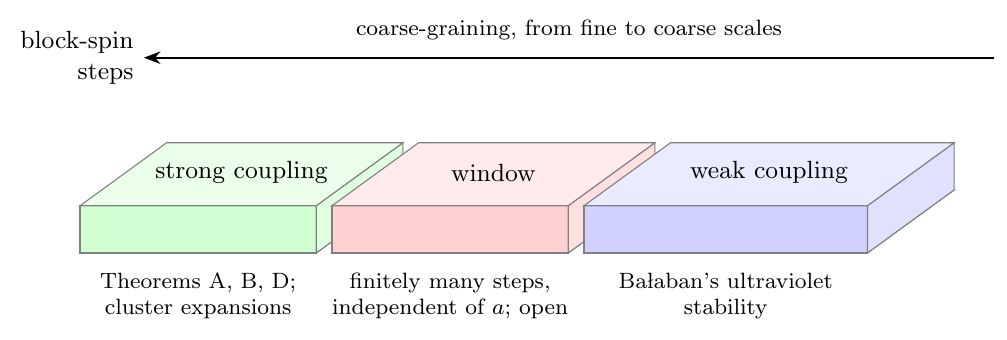
\includegraphics[width=0.95\textwidth]{figures/fig_scales.png}
\caption{The three regimes of the block-spin flow. The strong-coupling end is
controlled by the results of this paper and by cluster expansions, the
weak-coupling end by Ba{\l}aban's ultraviolet stability. No method controls the
window between them.}
\label{fig:scales}
\end{figure}

\begin{problem}[Crossover]\label{prob:crossover}
Show that at a block scale $a_*=c_*/\Lambda$ the effective density of the
four-dimensional $\SU(N)$ Wilson theory is a Wilson weight with coupling in
the regime of Theorem~B (or of a convergent cluster expansion) times
$\exp\sum_X\mathcal E_a(X)$, with $\mathcal E_a$ gauge invariant, local, and
small in the supremum norm over all block configurations, uniformly in the
spacing $a$ and in the volume.
\end{problem}

A solution of Problem~\ref{prob:crossover}, followed by the strong-coupling
analysis on the block lattice and reflection positivity of the fine theory,
would give a transfer-matrix gap of at least $ma$ at spacing $a$ with $m$
independent of $a$, which is the lattice form of the mass gap~\cite{BB26}; it
would also give a gap at every fixed coupling, by Proposition~\ref{prop:uniform}.
Problem~\ref{prob:crossover} is open. The tools of this paper do not reach it:
Theorem~C and Proposition~\ref{prop:ceiling} show that the curvature and
single-link Dobrushin methods stop at fixed small couplings because their
extremal configurations (all plaquettes equal to $z$, or zero staple sum) are
allowed, and Lemma~\ref{lem:stability} shows that feeding the corrections
$\mathcal E_a$ into a finite-box criterion needs a smallness that shrinks with
the box. The nearest test case, the crossover of the two-dimensional $\mathrm
O(3)$ sigma model at weak coupling, is itself unsettled by refereed work, and
three-dimensional $\SU(2)$ theory at large $\beta$ is open as well.

\section*{Data and code availability}

All proofs in this paper are by hand. The identities of
Lemma~\ref{lem:local}, the extremal values in Theorem~A and the Barta
computations of Lemma~\ref{lem:vmf} were also checked independently in exact
arithmetic, and the bound of Theorem~A against the numerically computed
Hessian on random configurations; these checks are archived with the source of
this paper in the repository \texttt{creelie/4Y-M}. The computations and checks
were carried out by Deep Bhattacharjee in Python (SymPy, NumPy, SciPy) with AI
assistance from Claude (Anthropic); both authors approved the final text.

\section*{Funding and competing interests}

The authors received no funding for this work and declare no competing
interests.

\begin{thebibliography}{99}

\bibitem{BE85}
D.~Bakry and M.~\'Emery, Diffusions hypercontractives, in \emph{S\'eminaire
de Probabilit\'es XIX}, Lecture Notes in Math. 1123, Springer, Berlin, 1985,
177--206, \href{https://doi.org/10.1007/BFb0075847}{doi:10.1007/BFb0075847}.

\bibitem{BGL14}
D.~Bakry, I.~Gentil and M.~Ledoux, \emph{Analysis and Geometry of Markov
Diffusion Operators}, Grundlehren Math. Wiss. 348, Springer, Cham, 2014,
\href{https://doi.org/10.1007/978-3-319-00227-9}{doi:10.1007/978-3-319-00227-9}.

\bibitem{Bal87}
T.~Ba{\l}aban, Renormalization group approach to lattice gauge field theories.
I, Comm. Math. Phys. \textbf{109} (1987), 249--301,
\href{https://doi.org/10.1007/BF01215223}{doi:10.1007/BF01215223}.

\bibitem{Bal88}
T.~Ba{\l}aban, Convergent renormalization expansions for lattice gauge
theories, Comm. Math. Phys. \textbf{119} (1988), 243--285,
\href{https://doi.org/10.1007/BF01217741}{doi:10.1007/BF01217741}.

\bibitem{Bar37}
J.~Barta, Sur la vibration fondamentale d'une membrane, C. R. Acad. Sci.
Paris \textbf{204} (1937), 472--473.

\bibitem{BB26}
D.~Bhattacharjee and U.~Bhattacharya, Spacing-uniform lattice inequalities
cannot produce the Yang--Mills mass gap, Zenodo, release v1.0.0, 2026,
\href{https://doi.org/10.5281/zenodo.23444338}{doi:10.5281/zenodo.23444338}.

\bibitem{BSB26}
D.~Bhattacharjee, P.~Samal and S.~Bhattacharya, Geometric structure and
renormalization group flow in chiral Yang--Mills--Higgs theory, Preprints
(2026), \href{https://doi.org/10.20944/preprints202602.2022.v1}
{doi:10.20944/preprints202602.2022.v1}.

\bibitem{BTBS26}
D.~Bhattacharjee, S.~N.~Thakur, S.~Bhattacharya and P.~Samal, SU($n$)
holonomy deviations in Calabi--Yau manifolds (CY1--CY4), Preprints (2026),
\href{https://doi.org/10.20944/preprints202602.0023.v1}
{doi:10.20944/preprints202602.0023.v1}.

\bibitem{CNS25b}
S.~Cao, R.~Nissim and S.~Sheffield, Dynamical approach to area law for lattice
Yang--Mills, \href{https://arxiv.org/abs/2509.04688}{arXiv:2509.04688}.

\bibitem{Cha21}
S.~Chatterjee, A probabilistic mechanism for quark confinement, Comm. Math.
Phys. \textbf{385} (2021), 1007--1039,
\href{https://doi.org/10.1007/s00220-021-04086-y}{doi:10.1007/s00220-021-04086-y}.

\bibitem{Dob70}
R.~L.~Dobrushin, Prescribing a system of random variables by conditional
distributions, Theory Probab. Appl. \textbf{15} (1970), 458--486,
\href{https://doi.org/10.1137/1115049}{doi:10.1137/1115049}.

\bibitem{DS85}
R.~L.~Dobrushin and S.~B.~Shlosman, Constructive criterion for the uniqueness
of Gibbs field, in \emph{Statistical Physics and Dynamical Systems},
Birkh\"auser, Boston, 1985, 347--370,
\href{https://doi.org/10.1007/978-1-4899-6653-7_20}{doi:10.1007/978-1-4899-6653-7\_20}.

\bibitem{DSa23}
T.~C.~Dorlas and B.~Savoie, On the Wasserstein distance and the Dobrushin
uniqueness theorem, \href{https://arxiv.org/abs/2305.19371}{arXiv:2305.19371}.

\bibitem{Fol82}
H.~F\"ollmer, A covariance estimate for Gibbs measures, J. Funct. Anal.
\textbf{46} (1982), 387--395,
\href{https://doi.org/10.1016/0022-1236(82)90053-2}{doi:10.1016/0022-1236(82)90053-2}.

\bibitem{FS82}
J.~Fr\"ohlich and T.~Spencer, Massless phases and symmetry restoration in
abelian gauge theories and spin systems, Comm. Math. Phys. \textbf{83} (1982),
411--454, \href{https://doi.org/10.1007/BF01213610}{doi:10.1007/BF01213610}.

\bibitem{Gut80}
A.~H.~Guth, Existence proof of a nonconfining phase in four-dimensional U(1)
lattice gauge theory, Phys. Rev. D \textbf{21} (1980), 2291--2307,
\href{https://doi.org/10.1103/PhysRevD.21.2291}{doi:10.1103/PhysRevD.21.2291}.

\bibitem{Jen12}
R.~Jentzsch, \"Uber Integralgleichungen mit positivem Kern, J. Reine Angew.
Math. \textbf{141} (1912), 235--244,
\href{https://doi.org/10.1515/crll.1912.141.235}{doi:10.1515/crll.1912.141.235}.

\bibitem{Kal21}
O.~Kallenberg, \emph{Foundations of Modern Probability}, 3rd ed., Springer,
Cham, 2021, \href{https://doi.org/10.1007/978-3-030-61871-1}
{doi:10.1007/978-3-030-61871-1}.

\bibitem{Lev03}
T.~L\'evy, Yang--Mills measure on compact surfaces, Mem. Amer. Math. Soc.
\textbf{166} (2003), no.~790,
\href{https://doi.org/10.1090/memo/0790}{doi:10.1090/memo/0790}.

\bibitem{Mig75}
A.~A.~Migdal, Recursion equations in gauge field theories, Sov. Phys. JETP
\textbf{42} (1975), 413--418.

\bibitem{Nis25}
R.~Nissim, U($N$) lattice Yang--Mills in the 't~Hooft regime,
\href{https://arxiv.org/abs/2510.22788}{arXiv:2510.22788}.

\bibitem{OSei78}
K.~Osterwalder and E.~Seiler, Gauge field theories on a lattice, Ann. Physics
\textbf{110} (1978), 440--471,
\href{https://doi.org/10.1016/0003-4916(78)90039-8}{doi:10.1016/0003-4916(78)90039-8}.

\bibitem{Sei82}
E.~Seiler, \emph{Gauge Theories as a Problem of Constructive Quantum Field
Theory and Statistical Mechanics}, Lecture Notes in Phys. 159, Springer,
Berlin, 1982, \href{https://doi.org/10.1007/3-540-11559-5}{doi:10.1007/3-540-11559-5}.

\bibitem{SSZ26}
H.~Shen, R.~Zhu and X.~Zhu, Langevin dynamics of lattice Yang--Mills--Higgs and
applications, Comm. Math. Phys. \textbf{407} (2026),
\href{https://doi.org/10.1007/s00220-025-05528-7}{doi:10.1007/s00220-025-05528-7}.

\bibitem{SZZ23}
H.~Shen, R.~Zhu and X.~Zhu, A stochastic analysis approach to lattice
Yang--Mills at strong coupling, Comm. Math. Phys. \textbf{400} (2023),
805--851, \href{https://doi.org/10.1007/s00220-022-04609-1}{doi:10.1007/s00220-022-04609-1}.

\bibitem{Wil74}
K.~G.~Wilson, Confinement of quarks, Phys. Rev. D \textbf{10} (1974),
2445--2459, \href{https://doi.org/10.1103/PhysRevD.10.2445}{doi:10.1103/PhysRevD.10.2445}.

\end{thebibliography}

\end{document}
